\documentclass[border=2pt]{standalone}
\usepackage{amsmath}
\usepackage{tikz}
\usetikzlibrary{matrix, shapes.geometric, shapes.misc, calc}
% Entry (1, 1): first row of A (teal) dotted with first column of B (red).
% Unfilled entries default to placeholder dots (see matrix-product.tikz).
\newcommand{\ra}[1]{\textcolor{mfpateal}{#1}}
\newcommand{\cb}[1]{\textcolor{mfpared}{#1}}
\newcommand{\sAA}{\ra{2} \cdot \cb{1} + \ra{10} \cdot (\cb{-1}) + \ra{0} \cdot \cb{1} + \ra{1} \cdot (\cb{-1})}
\newcommand{\pAA}{-9}
\newcommand{\punct}{.}
\begin{document}
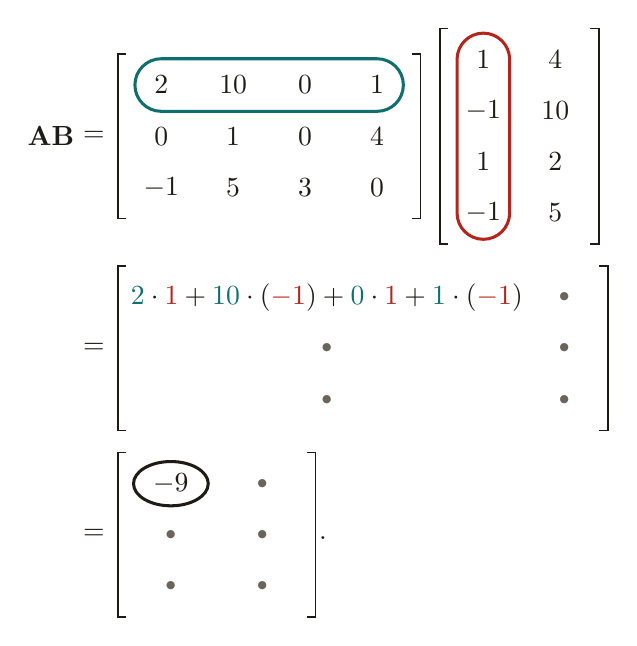
\begin{tikzpicture}
% Shared drawing of the matrix multiplication example in linear_algebra.qmd
% (@sec-matrix-multiplication), laid out like an align with the = signs lined up:
%
%   AB = [A][B]
%      = [sums]      (dot-product arithmetic)
%      = [product]   (the resulting numbers)
%
% \input by matrix-product*.tex so annotated versions can never drift apart.
% Not built on its own: build.sh only compiles *.tex.
%
% Entries of the two 3x2 matrices are macros, named by row letter then column
% letter: \sAA ... \sCB for the arithmetic line, \pAA ... \pCB for the product
% line. Define the ones a version fills in before \input; the rest default to a
% muted placeholder dot.
%
% Define \punct (e.g. as a period) if the display ends a sentence.
%
% Colours mirror the mfpa palette (_common.R / mfpa.scss).
\definecolor{mfpaink}{HTML}{1E1B16}
\definecolor{mfpateal}{HTML}{0F6E6E}
\definecolor{mfpared}{HTML}{B3261E}
\definecolor{mfpagreen}{HTML}{2E7D46}
\definecolor{mfpamuted}{HTML}{6B645A}
\providecommand{\blank}{\textcolor{mfpamuted}{{\scriptstyle\bullet}}}
\providecommand{\sAA}{\blank}\providecommand{\sAB}{\blank}
\providecommand{\sBA}{\blank}\providecommand{\sBB}{\blank}
\providecommand{\sCA}{\blank}\providecommand{\sCB}{\blank}
\providecommand{\pAA}{\blank}\providecommand{\pAB}{\blank}
\providecommand{\pBA}{\blank}\providecommand{\pBB}{\blank}
\providecommand{\pCA}{\blank}\providecommand{\pCB}{\blank}
\providecommand{\punct}{}
\tikzset{
  % Uniform ring around a single entry.
  entry ring/.style={draw=#1, ellipse, line width=1.1pt,
    minimum width=2.7em, minimum height=1.6em, inner sep=0pt},
  % Shared look of the matrices.
  mat/.style={matrix of math nodes, text=mfpaink, inner sep=0.45em,
    nodes={anchor=center, minimum height=1.3em, minimum width=2.2em, inner sep=0pt},
    column sep=0.4em, row sep=0.55em},
  % An = sign, centred vertically on the matrix to its right.
  eqsign/.style={text=mfpaink, inner sep=0pt},
}
% Ring a run of entries (a whole row or column): #1 colour, #2 first entry,
% #3 last entry. A pill rather than an ellipse, since an ellipse long enough to
% clear the end entries of a run overshoots the brackets.
\newcommand{\ringrun}[3]{%
  \path let \p1 = ($(#3) - (#2)$),
            \n1 = {atan2(\y1, \x1)},
            \n2 = {veclen(\x1, \y1)} in
    node[draw=#1, rounded rectangle, line width=1.1pt, rotate=\n1,
         minimum width=\n2 + 1.9em, minimum height=1.9em, inner sep=0pt]
    at ($(#2)!0.5!(#3)$) {};}
% Brackets drawn as plain strokes: TeX's extensible delimiters leave visible
% seams between their pieces once rasterized.
\newcommand{\brackets}[1]{%
  \draw[mfpaink, line width=0.55pt]
    ([xshift=0.3em]#1.north west) -- (#1.north west) -- (#1.south west) -- ([xshift=0.3em]#1.south west);
  \draw[mfpaink, line width=0.55pt]
    ([xshift=-0.3em]#1.north east) -- (#1.north east) -- (#1.south east) -- ([xshift=-0.3em]#1.south east);}

% Line 1: AB = [A][B]. The = sign at the origin is the alignment point.
\node[eqsign] (eq1) at (0, 0) {$=$};
\node[text=mfpaink, anchor=east, inner sep=0pt] at ([xshift=-0.28em]eq1.west) {$\mathbf{A} \mathbf{B}$};
\matrix (a) [mat, anchor=west] at ([xshift=0.45em]eq1.east) {
  2  & 10 & 0 & 1 \\
  0  & 1  & 0 & 4 \\
  -1 & 5  & 3 & 0 \\
};
\matrix (b) [mat, anchor=west] at ([xshift=0.7em]a.east) {
  1  & 4  \\
  -1 & 10 \\
  1  & 2  \\
  -1 & 5  \\
};
% Line 2: = [arithmetic].
\matrix (s) [mat, anchor=north west] at ([xshift=0.45em, yshift=-0.8em]eq1.east |- b.south) {
  \sAA & \sAB \\
  \sBA & \sBB \\
  \sCA & \sCB \\
};
\node[eqsign] (eq2) at (eq1 |- s.center) {$=$};
% Line 3: = [product].
\matrix (c) [mat, nodes={minimum width=2.9em}, anchor=north west] at ([xshift=0.45em, yshift=-0.8em]eq1.east |- s.south) {
  \pAA & \pAB \\
  \pBA & \pBB \\
  \pCA & \pCB \\
};
\node[eqsign] (eq3) at (eq1 |- c.center) {$=$};
\brackets{a}
\brackets{b}
\brackets{s}
\brackets{c}
% Sentence-ending punctuation, on the last matrix's middle-row baseline as TeX
% would set it.
\node[text=mfpaink, anchor=base west, inner sep=0pt]
  at ([xshift=0.12em]c.east |- c-2-1.base) {\punct};

\ringrun{mfpateal}{a-1-1}{a-1-4}
\ringrun{mfpared}{b-1-1}{b-4-1}
\node[entry ring=mfpaink] at (c-1-1) {};
\end{tikzpicture}
\end{document}
